\section{Method} \label{sec:method}

In this Section we will describe the method we have used to solve the authorship
verification problem presented in Definition \ref{def:authorship_verification}.
In general there are two methods of representing each author. There is the
\textit{instance based approach} and the \textit{profile based approach}. In
the instance based approach each author $\alpha \in \mathcal{A}$ is represented
by a set of texts they have written $T_\alpha$. In the profile based approach
texts of $T_\alpha$ are combined in some way, resulting in a single (typically
smaller) ``profile'' representing the author. The instance based approach is
illustrated in Figure \ref{fig:instance_based} and the profile based approach is
illustrated in Figure \ref{fig:profile_based}.

\begin{figure}[htb]
    \centering
    \textbf{Instance Based Authorship Verification or Authorship Attribution}\par\medskip
    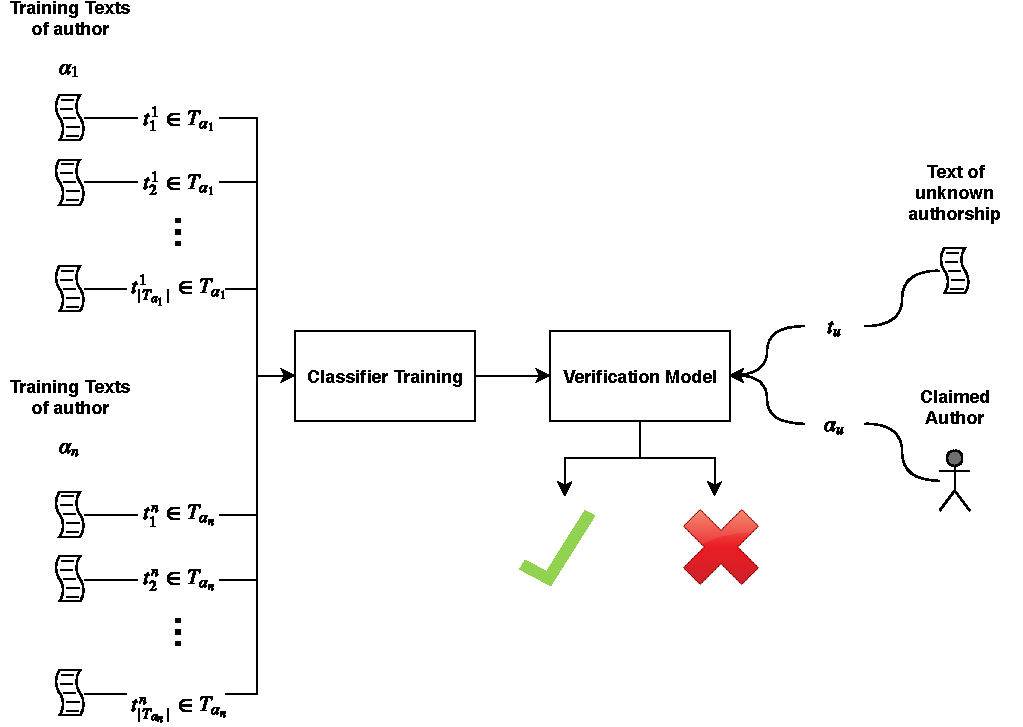
\includegraphics[scale=0.5]{./pictures/method/instance_based}
    \caption{Illustrate the typical instance based authorship verification or
        authorship attribution solution setup. Inspired by \citet{stamatos2009}
        a set of authors are given as input each with a set of texts. Some
        machine learning model is trained on the input texts and the model is
        used to predict an unknown text.}
    \label{fig:instance_based}
\end{figure}

\begin{figure}[htb]
    \centering
    \textbf{Profile Based Authorship Verification or Authorship Attribution}\par\medskip
    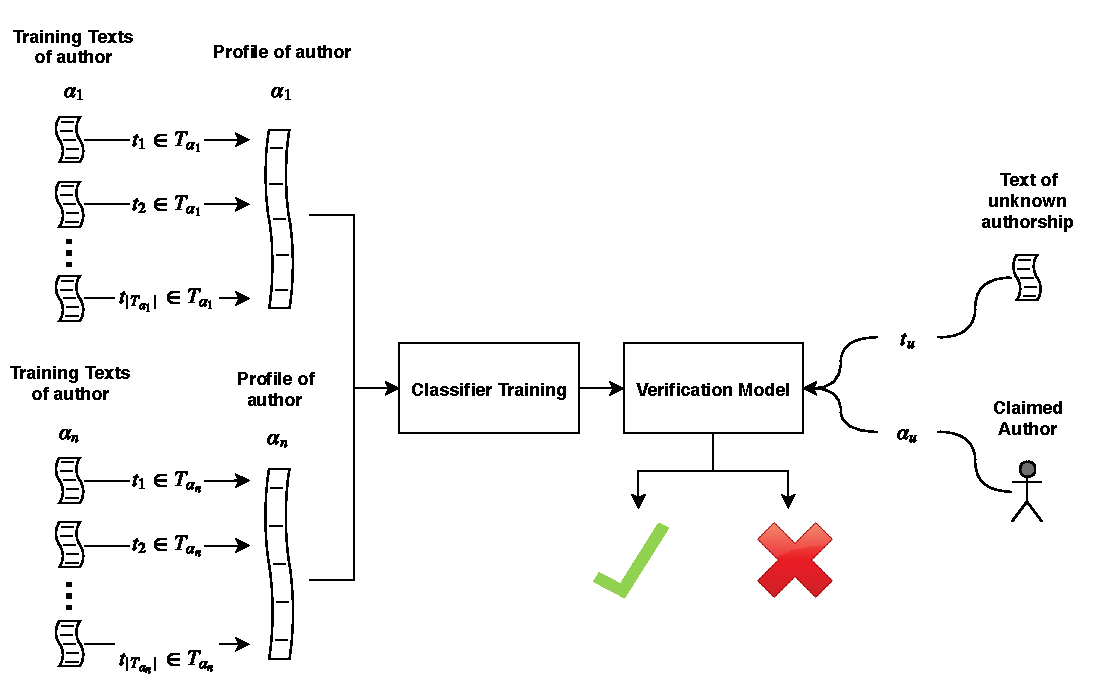
\includegraphics[scale=0.5]{./pictures/method/profile_based}
    \caption{Illustrate the typical profile based Authorship Verification or
        Authorship Attribution setup. Inspired by \citet{stamatos2009} the texts
        of each author are combined using some combination function such as an
        average or a concatenation. Those \textit{profiles} are then given to a
        Machine Learning model to train. The output is a model which is used to
        predict unknown texts.}
    \label{fig:profile_based}
\end{figure}

An example of a profile-based authorship attribution approach, which is highly
regarded by \citet{stamatos2009} use of a compression algorithm. It works not by
representing each author profile as a set of features, but rather makes use of
compression to do so. In the initial scenario we have a set of author-profiles
which is the concatenation of all their individual work. When a new text is then
introduced the authorship is determined by looping through each author adding
it to their concatenated profile. The profile is then compressed both with
and without the new text included. The bit-wise difference is then computed,
by subtracting them from one another resulting in what is essentially the
cross-entropy between the two sets. The author with the lowest cross-entropy
is then considered to be the author of this new text. Different methods of
comprehension can be used as the base for this model each giving different
results. In the instance that \citet{stamatos2009} describes, RAR compression
yielded the best results, but the choice of compression algorithm depends on the
specific scenario.

We will generally use the instance based approach since it allows us to use
more metadata text information. For example the writing style of author may
change over time especially for secondary school pupils that evolve very much
in a short amount of time. Since we use an instance based approach we are able
to weight similarity to newer texts higher than similarity to older texts as
\citet{hansen2014} found worked well. The practical application of this, will be
explained in Section \ref{subsec:combining_neural_network_output}.

There are also another split between methods that we consider. There are
generalizing and author specific models. In a generalizing model only a single
model is trained on data from multiple authors and are able to make predictions
about previously unseen authors. In the author specific model a separate model
has to be trained for each author and is not able to make predictions for
previously unseen authors. The generalizing models main advantage is that it
only has to be trained once and after that it can be used for everyone and it
can make use of a large amount data since it can use data from several authors
for training. The author specific model has the advantage that it can better fit
to the specific quirks of a particular author since it is trained separately
for each author. The downside of the author specific approach is that a new
model has to be trained for each new author. We will focus on the generalizing
approach since it is easier to implement for MaCom as they only have to train a
model once.

As a unit of measuring the quality of our models, we will also compute the
number of \glspl{TP}, \glspl{TN}, \glspl{FP} and \glspl{FN}, as seen in
\citet{US}. In these problems we get,

\begin{itemize}
    \item a \gls{TP} whenever we answer \textit{True} and the texts are written
        by the same author,
    \item a \gls{TN} whenever we answer \textit{False} and the texts are
        \textbf{not} written by the same author,
    \item a \gls{FP} whenever we answer \textit{True} and the texts are
        \textbf{not} written by the same author,
    \item a \gls{FN} whenever we answer \textit{False} and the texts are written
        by the same author.
\end{itemize}

Given those definitions the \gls{TPR}, \gls{FPR}, \gls{TNR} and \gls{FNR}
describes.

\begin{description}
    \item[\gls{TPR}: ]

        The fraction of positives that we reported \textit{True} on i.e. the
        fraction of texts written by the same author that we say are written by
        the same author.

    \item[\gls{TNR}: ]

        The fraction of negatives that we reported \textit{False} on i.e. the
        fraction of texts written by different authors that we say are written
        by different authors.

    \item[\gls{FPR}: ]

        The fraction of negatives that we reported \textit{True} on i.e. the
        fraction of texts written by different authors that we say are written
        by the same author.

    \item[\gls{FNR}: ]

        The fraction of positives that we reported \textit{False} on i.e. the
        fraction of texts written by the same author that we say are written by
        different authors.

\end{description}

And they can be computed as,

\begin{align}
    TPR &= \frac{TP}{TP + FN}, \\
    FPR &= \frac{FP}{FP + TN}, \\
    TNR &= \frac{TN}{TN + FP}, \\
    FNR &= \frac{FN}{FN + TP}.
\end{align}

Using these definition we can also describe the accuracy measure we will be
reporting on throughout our experiments,

\begin{equation}
    \text{Accuracy} = \frac{TP + TN}{TP + FP + TN + FN}.
\end{equation}

In the case of MaCom, we want to minimize the \gls{FNR} as much as possible,
so as to not wrongfully accuse anyone of not having written their assignment.
This however leaves out a equally important metric. While a low \gls{FNR} is
the goal, MaCom also wants to minimize the number of \glspl{FN} compared to the
total number of accusations made. This can be described as:

\begin{equation}
    \text{Accusation Error} = \frac{FN}{FN + TN}.
\end{equation}

The goal is also to keep this error under a certain threshold specified
by MaCom, which in this case is $0.1$ or $10\%$. In other words, of the
accusations we made, only $10\%$ of them are allowed to be wrong. In order
to accommodate this constraint we can take certain actions which depends on
the model used. Details about these actions will be addressed in Section
\ref{subsec:combining_neural_network_output}.

In addition to the constraint on the accusation error Macom also wants a
specificity of above 95\%. Specificity is defined as,

\begin{equation}
    \text{Specificity} = \frac{TN}{(TN + FP)}.
\end{equation}

Specificity therefore represents the fraction of the total negatives we catch.
To catch 95\% of ghost writers is a very ambitious goal. As described earlier it
is more important to keep the accusation error low than to catch many ghost
writers. We will therefore primarily focus on keeping the accusation error lower
than 10\% and then see how high we can get the specificity at the same time.

\subsection{Baseline Methods}

We have implemented two baselines to compare with our neural network methods.
The methods are based on work by \citep{US}. The methods were developed for
English texts and not Danish texts that we work with in this assignment. They do
however represent classical machine learning methods for solving the authorship
verification problem. They will therefore serve as a great baseline for our
neural networks. We believe that by changing the parameters of the models
they will work just as well for Danish texts that they did on English texts.
The Danish and English language is very similar as they both derive from the
Germanic branch of the indo-European language family. \citet{konstantin:2000}
conducted a study of the similarities and differences between different European
languages. They found that as expected Danish and English were very close.

None of the baseline methods works on raw texts. Rather they require hand
engineered feature sets extracted from the texts. The features used by
\citet{US} were all n-gram frequencies which is similar to classic authorship
verification methods \citep{stamatos2009}. We use the same features as described
in the project. We change the specific n-grams to n-grams extracted from Danish
texts but the classes of n-grams will stay the same. The n-grams come from
several linguistic layers. Specifically we use frequencies of character-n-grams,
special-character-n-grams, word-n-grams and \gls{POS}-tag-n-grams.

\begin{description}

    \item[Character-n-gram]

        Refer to character sequences of size $n$.

    \item[Special-character-n-grams]

        Refer to sequences of characters of size $n$ where all alphanumeric and
        space characters has been removed from a text. Special-character-n-grams
        can for example be used to find authors that use long sentences and
        therefore many commas in a row.

    \item[Word-n-grams]

        Refer to sequences of words of size $n$.

    \item[\gls{POS}-tag-n-grams]

        Refer to \gls{POS}-tag sequences of size $n$. A \gls{POS}-tag is the
        grammatical class of individual words such as nouns of adjectives. To
        extract \gls{POS}-tags from texts we use the \gls{POS}-tagger provided
        by \citep{polyglot}.

\end{description}

We will now describe shortly the two baseline methods we implemented. For
details on the methods see \citep{US}.


\subsubsection{Extended Delta Method}

One of the best performing methods of \citet{US} was the extended delta method.
As the name suggests the method extends the already existing delta method
\citep{evert2015towards}. The original delta method verifies authorship of
a text by finding the nearest text to a queried text in a feature set. If
the nearest text is written by the candidate author the method reports true
and otherwise false. The features used in the original delta method were the
frequencies of the 300 most frequent words \citep{evert2015towards}.

The extended delta method is an extension to that method. In this method we are
allowed to change the distance metric used to compare feature vectors, the
features used and the number of nearest neighbours to consider. Since we can
change the number of nearest neighbours to consider we are now using a \gls{KNN}
classifier with a custom comparison function.

Like \citet{US} we will find the best parameters via cross validation. We will
try 5 distance metrics. The 5 distance metrics will be the Minkowski distance
with $p = 1 \dots 5$. When $p = 1$ the distance metric is the manhattan distance
and when $p = 1$ the euclidian distance. We chose the manhattan distance since
it has been shown to consistently perform well when compared to other distance
metrics \citep{evert2015towards}. And we chose the Euclidean metric since it has
been shown to work well on a small amount of features \citep{evert2015towards}.
The rest of the $p$ values are there or seeing if we could find something better
than the classical distance metrics. The different number of nearest neighbours
we will try will initially be between 1 and 15. However if we find that 15 gives
the best results we will expand the search to more than 15.


\subsubsection{Author Specific SVM}

Our other baseline method is the author specific \gls{SVM}. The method
was used in \citep{US} and was originally inspired by \citet{hansen2014}.
They used the an \gls{SVM} on the Macom dataset as we described in Section
\ref{subsec:previous_work_using_macoms_dataset}. To verify the authorship of a
text $t$ and author $\alpha$ using this method, a two class \gls{SVM} classifier
have to be trained. The positive class is represented by features of each $t'
\in T_\alpha$ and the negative class is represented by the features of $t''
\in T\ |\ T \subset \overline{T_\alpha}, |T| = |T_\alpha|$. After training the
classifier is used to predict the text we are verifying the authorship of $t$.
Since a separate \gls{SVM} is trained for each author it can learn the specific
authors writing style from $T_\alpha$ supplied and in contrast what the writing
style of someone not him is.

The method is based on an \gls{SVM} so we have to experiment with the
hyperparameters $C$ and $\gamma$. We will find good parameters via cross
validation. The parameter search will be described in detail in Section
\ref{sec:experiments}.


\subsection{Deep Learning}

In this paper we will approach the authorship verification problem using
deep learning. The term deep learning, was first introduced to machine machine
learning in 1989, and afterward to \glspl{NN} in 2000. The terms quickly became
synonymous with \glspl{NN} due to them being some of the more efficient deep
learning methods \citep{Schmidhuber:2015}.

With the inner workings of the brain used as the basis, a standard simple
\gls{NN} consists of a set interconnected processors, called neurons. Each of
these neurons has a real valued activation associated with it, which activates
differently depending on the specific neuron. The input neurons activate
through perceiving the environment, or in other words, when they are fed data
externally. Other neurons are simply activated through the weighted activation
of previous neurons \citep{DBLP:journals/corr/Schmidhuber14}.

\glspl{NN} have been around since the 1940s. However, back then they were
merely variations of the linear regressors used at the time, and was not
very reminiscent of the networks on can see today. It was not until the late
1960s, early 1970s, that networks comparable to the more modern approaches
surfaced. Examples of such early works are \citep{ivakhnenko1973cybernetic} and
\citep{4308320}, which describe multi-layered feed forward supervised neural
network architectures. While the work described in \citep{4308320} was indeed
one of the first cases of the modern \gls{NN}, getting the network to learn was
still a problem, as the tweaking of individual weights attributed to each neuron
in the network was not trivial. Little did they know, research to solve that
problem was already in progress. The basics of continuous \gls{BP} was initially
described in 1960, by \citet{Kelley1960}, quickly followed by a simpler approach
which used only the chain rule in 1962 by \citet{DREYFUS196230}. It was not
until 1970 that the modern version of \gls{BP} was described, using automatic
differentiation as its basis. This prompted an increase in \gls{BP} related
research in the following decades. As computational power increased in the
1990s and 2000s, so did the practical usage of \gls{BP}, and \gls{NN} in
general \citep{Schmidhuber:2015}. The real life application of \gls{BP} will be
described in Section \ref{subsubsec:training_a_network}.

Like with the history of authorship attribution research in this area of science
picked up more interest as we entered the modern computational age, and with
the introduction of the \gls{CNN}. \glspl{CNN} are based on the early work
described in \citet{TJP:TJP19681951215}. They showed that cats and monkeys
visual cortexes contain a set of neurons, each individually responding to a
receptive field, or area, of their field of view. Neighboring receptive fields
all have a certain amount of overlap but in the end a cohesive view is created.
This is what paved the way for neocognition in 1980 \citep{Fukushima1980}, the
basis of \glspl{CNN} which works in a very similar manner looking at overlapping
subsections of data. These convolutional neurons however were rarely used alone
but together with a down-sampling neuron such as Max Pooling introduced in 1993
\citep{Schmidhuber:2015}.


\subsubsection{Neurons}\label{sec:neurons}

As mentioned previously a \gls{NN} consists of a collection of neurons. Each
neuron is a simplified mathematical model which behaves much like neurons in
the brain. They receive, process and transmit information. Each neuron has a
set of inputs called $x_{j}$ one of which $x_{0}$ is a special bias input set
to 1 and a single output called $z_i$, where $i$ refers to the neuron and $j$
refers to the specific input to that neuron. Each neuron computes a weighted sum
of its inputs and applies an activation function $h$ to the weighted sum. The
weights are called $w_{ij}$ and the weight of the bias $w_{i0}$. The function
each neuron computes is,

\begin{equation}\label{eq:neuron}
    z_i = h(a_i) = h\left(
        \sum_{j = 1}^d w_{ij}x_j + w_{i0}
 \right) = h\left(
        \sum_{j = 0}^d w_{ij}x_j \right)
\end{equation}

where $d$ is the number of inputs to the neuron. A more intuitive model of such
a neuron can be seen in Figure \ref{fig:neuron}.

\begin{figure}[!tbp]
  \centering
  \begin{minipage}[b]{0.45\textwidth}
    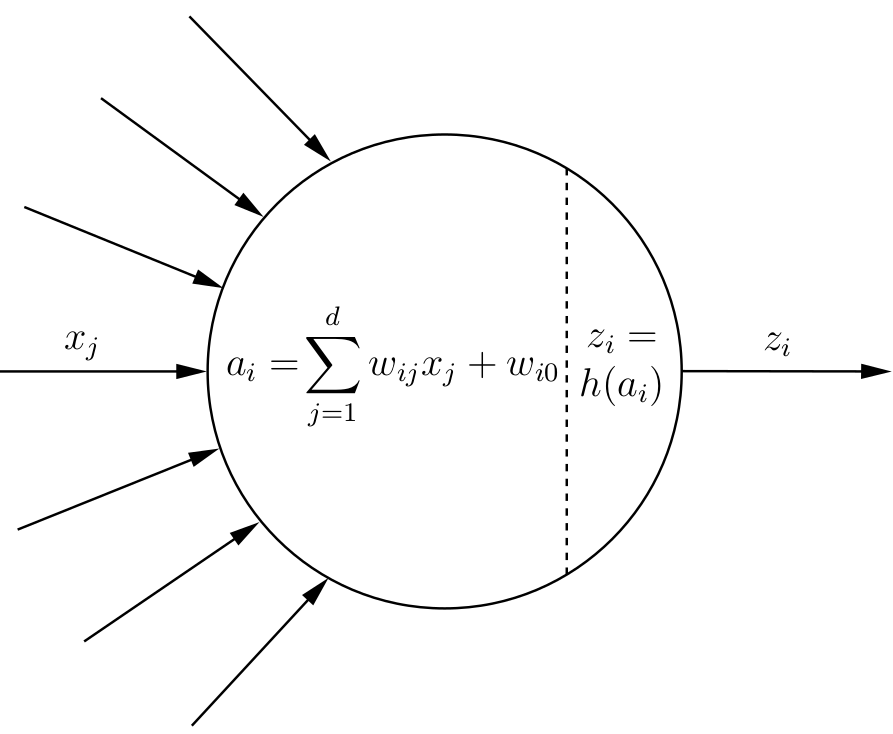
\includegraphics[width=\textwidth]{./pictures/method/neuron.png}
  \end{minipage}
  \hfill
  \begin{minipage}[b]{0.45\textwidth}
    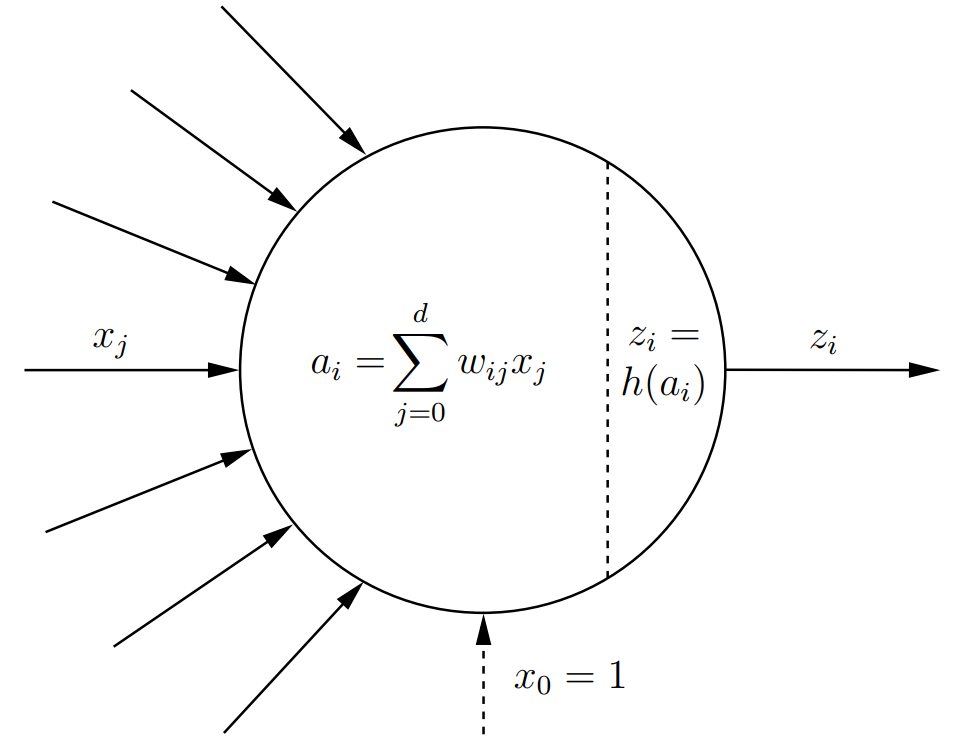
\includegraphics[width=\textwidth]{./pictures/method/neuron_bias.png}
  \end{minipage}
    \caption{The inner workings of a neuron, with and without an implicit
        bias \citep{Igel}. The left figure is without implicit bias while the
        right figure is with implicit bias.}
\label{fig:neuron}
\end{figure}

Neurons are usually arranged in layers in order to achieve a certain desired
behaviour, more details regarding these specific layers will be explained in
later chapters. The training of a \gls{NN} consists of changing the weights
applied at each neuron, with the goal of modeling the relationships present in
the data.


\subsubsection{Activation Functions} \label{subsubsec:activation_functions}

The activation function $h$, used at each neuron, defines the output of the
neuron given a certain input. A simple example of this would be computer chip
circuit, which can be seen as a series of activation functions outputting 0 or
1 depending on their input. This activation function would be a linear one.
When applying activation functions to neurons in \glspl{NN}, they are usually
non-linear, as it allows for the computation of more complex problems using a
smaller amount of neurons, relative to usage of a linear activation function,
as they allow for the universal function approximation, a point also made by
\citet{6797088} A plot of different activation functions is shown in Figure
\ref{fig:activation_functions}.

\begin{figure}
    \centering
    \textbf{Activation Functions}\par\medskip
    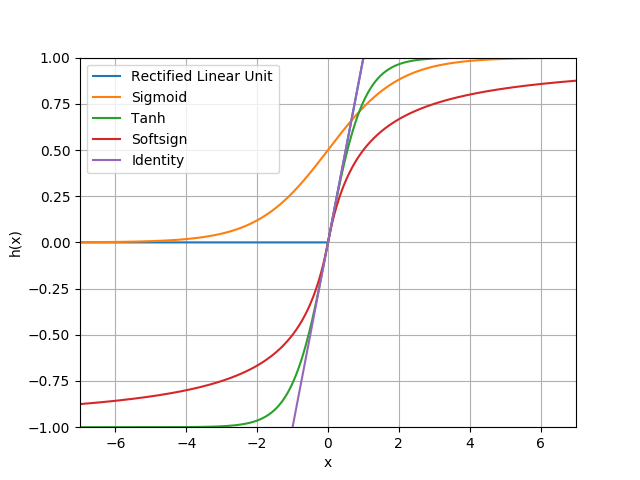
\includegraphics[width=0.5\textwidth]{./pictures/method/activation_functions.png}
    \caption{Different activation functions that can be used in neural
        networks.}
    \label{fig:activation_functions}
\end{figure}

Each activation function has its pros and cons. We mainly made use of the
\gls{ReLu} activation function in the hidden layers of our networks. The reason
for this selection is its general purpose use. When selecting an activation
function for your neurons, the best function would be the one which best
approximates the underlying data relationship. Without a good idea as to what
that function might be, \gls{ReLu} is a good starting point. Its simplicity
provides a quick computation time, and its below zero limitation means that
a large portion of the network will not be activating, resulting in an even
smaller computation time. In addition to that, the derivative of the function
is 1 in the case of a positive input, resulting in the \gls{BP} loss having
equal influence throughout the network. In the case of other activation
functions, this might not be the case, resulting in an altering of the error
as we propagate backwards through the network. This could lead to a big error
in the deeper layers not reaching the shallow layers of the network. This
property of the \gls{ReLu} activation function, does however not come without
its costs. If the learning rate of the network is not configured correctly, a
\gls{ReLu} activated neuron might be blasted with a gradient so large, that it
never reaches a point of activation again. In other words, the neuron "dies". As
such, one can risk a network containing a lot of dead non-activation neurons,
thus greatly decreasing its learning quality. On the other hand the sigmoid
function does not allow its neurons to die. It can become victim to saturation.
In the case of a weight being too small or too large, the output values will
be placed at the far ends of the sigmoid range of values. At this point the
gradient is incredibly small, meaning that the contribution that neuron now
has is negligible. This neuron is now only a strain on the network, slowing
it down through its activation but contributing nothing a problem \gls{ReLu}
does not have. Its based on these considerations we chose the \gls{ReLu}
activation function, leaving us the task of properly selecting our learning rate
\citep{JiYan, AndrejKarpathy, AvinashSharmaV}.

As the activation function of our output neurons we have used the softmax
function. The function is defined as

\begin{equation}
    h(x_i) = \frac{e^{x_i}}{\sum_{k=1}^n e^{x_k}}, \text{for $i = 1 \dots n$}.
\end{equation}

The softmax function takes any vector $x \in \mathbb{R}^n$ and returns a vector
$y \in [0, 1]^n$. Where the sum of the output vectors elements will be equal to
1. The function is therefore great at constructing a probability distribution
based on an input vector.

Exceptions to usage of the \gls{ReLu} activation function can be found when
we make use \gls{LSTM} layers during our experimentation. It makes use of the
tanh activation function,

\begin{equation}\label{eq:tanh}
h(x) = \tanh(x) = \frac{(e^x - e^{-x})}{(e^x + e^{-x})}
\end{equation}

and the hard sigmoid activation function

\begin{equation}\label{eq:h_sig}
h(x) = \max(0, \min(1, x \cdot 0.2 + 0.5))
\end{equation}

These both serve as the default activations functions when using the keras deep
learning library. \cite{chollet2015keras}

\subsubsection{Layers} \label{subsubsec:layers}

\glspl{NN} are organized in layers. The first layer is called the input layer
and is connected directly to the input to the model and the last layer is called
the output layer and gives the output of the model. All layers in between
are called hidden layers. A practical example could be where the input layer
was layer of neurons where each neuron is connected to a pixel in an input
image. And the output layer could consist of a single neuron that computes the
probability that the picture contained a cat. An example layered \gls{NN} are
shown in Figure \ref{fig:example_nn}.

\begin{figure}
    \centering
    \textbf{Example Neural Network}\par\medskip
    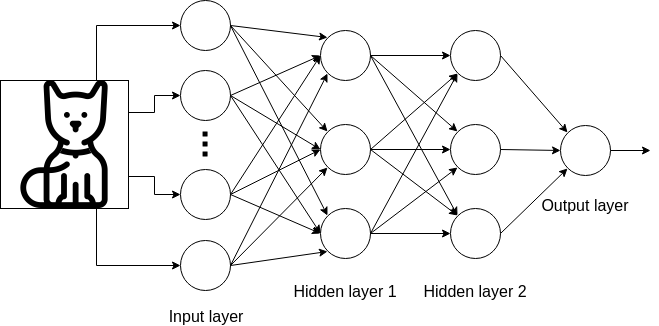
\includegraphics[width=\textwidth]{./pictures/method/example_neural_network}
    \caption{Example neural network that illustrates how neurons are organized
        into different layers with a special input layer, a special output layer
        and two hidden layers. The neurons in the input layer are connected to
        individual pixels in an input image and the output layer is a single
        neuron computing the probability that the image contains a cat.}
    \label{fig:example_nn}
\end{figure}

There are different kinds of layers. Below is a
non-exhaustive description of different layers, based on
\citep{oshea2015,DBLP:series/sci/2012-385,Goodfellow-et-al-2016,
mikolov2013linguistic,JMLR:v15:srivastava14a}.

\begin{description}

    \item[Dense Layer:]

        In a dense layer the input of each neuron in the layer is connected to
        the output of every neuron in the previous layer. Each neuron in the
        layer computes a weighted sum of the outputs of the previous layers'
        neurons and applies an activation function. The weights for each of
        the neurons in the layer are different allowing each neuron to learn a
        different combination of the previous layer. An example of this can be
        seen in Figure \ref{fig:example_nn}, where the hidden layers are Dense.

    \item[Convolutional Layer:]

        A convolutional layer is mainly used to extract position independent
        features from data. The convolution consist of a sliding window that
        slides over some input data and gives an output for each possible
        position in the input image. The sliding window uses the same weights
        in all the input and will therefore extract the same features from
        different locations if it is presented with the same input. The
        convolution computes a single output for each window position. The
        output is computed as the sum of the elementwise multiplication of
        the sliding window and the current part of the input it is looking at
        \citep{oshea2015}. Let us for example consider a two dimensional input,

        \begin{equation}
            X = \begin{pmatrix}
                1 & 1 & 1 & 0 \\
                1 & 0 & 0 & 1 \\
                0 & 1 & 0 & 1 \\
                0 & 0 & 1 & 0
            \end{pmatrix},
        \end{equation}

        and the convolutional filter,

        \begin{equation}
            w = \begin{pmatrix}
                1 & 0 & 0 \\
                1 & 0 & 0 \\
                0 & 1 & 0 \\
            \end{pmatrix}.
        \end{equation}

        Then we start the sliding window in the top left corner and compute the
        elementwise product of the matrices,

        \begin{equation}
            Y = X_{[1,3;1,3]} \otimes w =
            \begin{pmatrix}
                1 & 1 & 1 \\
                1 & 0 & 0 \\
                0 & 1 & 0
            \end{pmatrix} \otimes
            \begin{pmatrix}
                1 & 0 & 0 \\
                1 & 0 & 0 \\
                0 & 1 & 0
            \end{pmatrix} =
            \begin{pmatrix}
                1 & 0 & 0 \\
                1 & 0 & 0 \\
                0 & 1 & 0
            \end{pmatrix},
        \end{equation}

        to then compute the final value we take the sum of all the elements in
        that matrix,

        \begin{equation}
            \sum_{i,j} Y_{i,j} = 1 + 0 + 0 + 1 + 0 + 0 + 0 + 1 + 0 = 3.
        \end{equation}

        We then slide the window one to the right and repeat the same process,

        \begin{equation}
            Y = X_{[2,4;1,3]} \otimes w =
            \begin{pmatrix}
                1 & 1 & 0 \\
                0 & 0 & 1 \\
                1 & 0 & 1
            \end{pmatrix} \otimes
            \begin{pmatrix}
                1 & 0 & 0 \\
                1 & 0 & 0 \\
                0 & 1 & 0
            \end{pmatrix} =
            \begin{pmatrix}
                1 & 0 & 0 \\
                0 & 0 & 0 \\
                0 & 0 & 0
            \end{pmatrix},
        \end{equation}

        and the final value,

        \begin{equation}
            \sum_{i,j} Y_{i,j} = 1.
        \end{equation}

        We keep sliding the window right until we run out of input. After that
        we go back to the left and go one row down. We continue the process for
        all the input and we end up with the matrix,

        \begin{equation}
            O = \begin{pmatrix}
                \sum_{i,j} \left( X_{[1,3;1,3]} \otimes w \right)_{i,j} &
                \sum_{i,j} \left( X_{[2,4;1,3]} \otimes w \right)_{i,j} \\
                \sum_{i,j} \left( X_{[1,3;2,3]} \otimes w \right)_{i,j} &
                \sum_{i,j} \left( X_{[2,4;2,3]} \otimes w \right)_{i,j}
            \end{pmatrix} = \begin{pmatrix}
                3 & 1 \\
                1 & 2
            \end{pmatrix}.
        \end{equation}

        A visualization of this process can be seen in Figure
        \ref{fig:convolution_visualization}.

        \begin{figure}
        \centering
        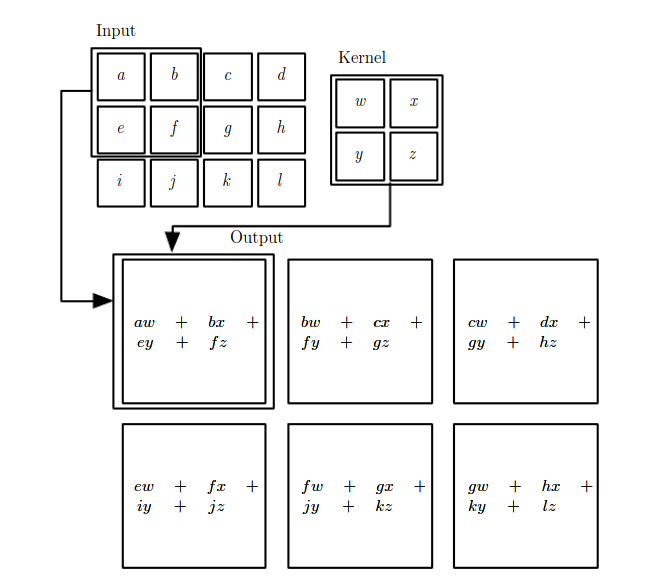
\includegraphics[width=0.6\textwidth]{./pictures/method/convolution_visualization.png}
        \caption{An example of 2D convolution, using a 2x2 kernel/sliding window
            size and a step size of 1 \citep{Goodfellow-et-al-2016}.}
        \label{fig:convolution_visualization}
        \end{figure}

        It can be seen that the output size is smaller than the input size. To
        prevent that the input can be padded with some value. A normal choice is
        zero padding. For the above input that would result in,

        \begin{equation}
            \begin{pmatrix}
                1 & 1 & 1 & 0 \\
                1 & 0 & 0 & 1 \\
                0 & 1 & 0 & 1 \\
                0 & 0 & 1 & 0
            \end{pmatrix} \xrightarrow{\text{zero padding}}
            \begin{pmatrix}
                0 & 0 & 0 & 0 & 0 & 0 \\
                0 & 1 & 1 & 1 & 0 & 0 \\
                0 & 1 & 0 & 0 & 1 & 0 \\
                0 & 0 & 1 & 0 & 1 & 0 \\
                0 & 0 & 0 & 1 & 0 & 0 \\
                0 & 0 & 0 & 0 & 0 & 0
            \end{pmatrix}.
        \end{equation}

        The sliding length can be different than one and is usually referred
        to as stride. The weights the convolutional window uses are learnable
        by the network. Certain convolutional filters can be used for
        edge detection and blurring the input. Some examples of different
        convolutional kernels applied to a grayscale image are shown in Figure
        \ref{fig:convolution_example}.

        \begin{figure}
            \centering
            \textbf{Examples of different convolutional kernels}\par\medskip
            \begin{tabular}{ccc}
                \textbf{Original} & \textbf{Kernel} & \textbf{Result} \\
                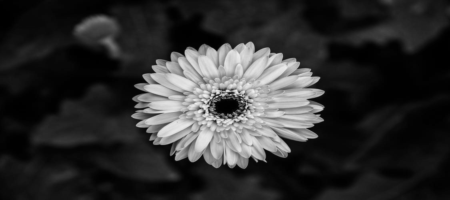
\includegraphics[width=0.3\textwidth]{./pictures/method/original_convolution.png} &
                \raisebox{1.2\height}{
                \begin{minipage}[b]{6cm}
                    \begin{equation*}
                        \begin{pmatrix}
                            1 & 0 & -1 \\
                            0 & 0 & 0  \\
                            -1 & 0 & 1
                        \end{pmatrix}
                    \end{equation*}
                \end{minipage}}
                    &
                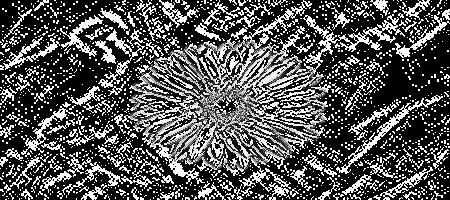
\includegraphics[width=0.3\textwidth]{./pictures/method/edge_detect_convolution.png} \\

                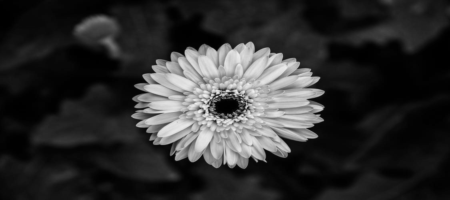
\includegraphics[width=0.3\textwidth]{./pictures/method/original_convolution.png} &
                \raisebox{1.2\height}{
                \begin{minipage}{6cm}
                    \begin{equation*}
                        \frac{1}{16}\begin{pmatrix}
                            1 & 2 & 1 \\
                            2 & 4 & 2  \\
                            1 & 2 & 1
                        \end{pmatrix}
                    \end{equation*}
                \end{minipage}}
                    &
                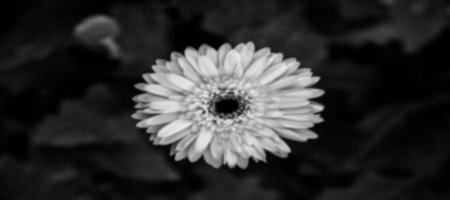
\includegraphics[width=0.3\textwidth]{./pictures/method/blurred_convolution.png} \\

                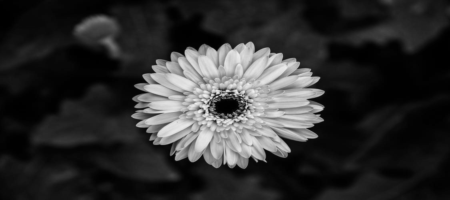
\includegraphics[width=0.3\textwidth]{./pictures/method/original_convolution.png} &
                \raisebox{1.2\height}{
                \begin{minipage}{6cm}
                    \begin{equation*}
                        \begin{pmatrix}
                            0  & -1 & 0  \\
                            -1 & 5  & -1 \\
                            0  & -1 & 0
                        \end{pmatrix}
                    \end{equation*}
                \end{minipage}}
                    &
                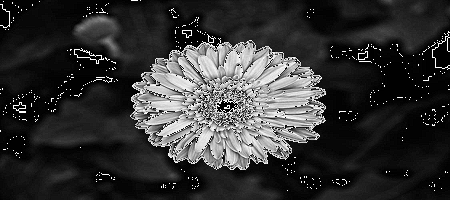
\includegraphics[width=0.3\textwidth]{./pictures/method/sharpened_convolution.png}
            \end{tabular}
            \caption{Examples of convolutional kernels applied to an image. The
                first kernel is an edge detect kernel, the second a blurring
                kernel and the third a sharpening kernel.}
            \label{fig:convolution_example}
        \end{figure}

        Convolutional layers for text analysis works slightly differently.
        Text is not two dimensional but one dimensional data. A convolution
        on text therefore does not use a two dimensional weight matrix but a
        weight vector. The process is the same as before. The weights vector
        slides over the text looking at a sequence of characters at a time. Each
        character is multiplied by the weight in that positition and a sum is
        computed. The output of the layer is a one dimensional sequence of these
        weighted sums. We will describe in more detail how convolutions for text
        work in Section \ref{subsubsec:conv_char_nn}.

    \item[\gls{RNN} Layer:]

        An \gls{RNN} network resembles a normal feed forward
        neural network except that it allows circular connections
        \citep{DBLP:series/sci/2012-385}. The circular connections can be used
        to remember previous inputs and an \gls{RNN} therefore has a sense of
        history of previous input and output. Classical feed forward neural
        networks can be viewed as mappings from and to vectors while \glspl{RNN}
        can be viewed as mappings from and to sequences. An \gls{RNN} does not
        view its input as a vector but as a sequence of inputs in different
        timesteps. We have shown an example of an \gls{RNN} network in Figure
        \ref{fig:rnn_illustration}.

        \begin{figure}
            \centering
            \textbf{Illustration of an \gls{RNN} Layer}\par\medskip
            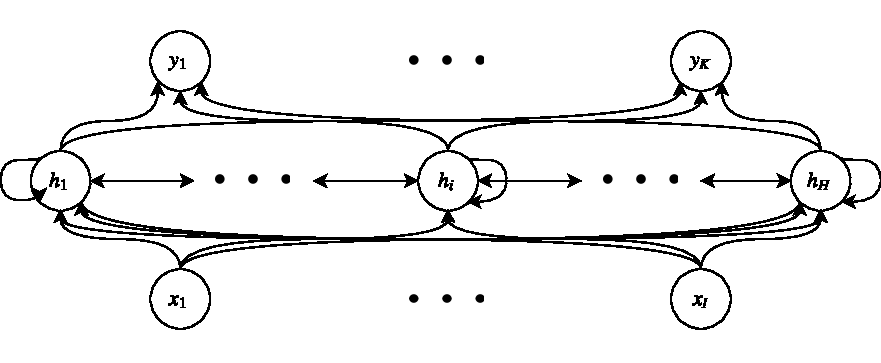
\includegraphics[width=\textwidth]{./pictures/method/RNN}
            \caption{Illustrates the structure of an \gls{RNN}. The \gls{RNN}
                consist of three layers, an input layer, a hidden layer and an
                output layer. The \gls{RNN} shown consist of $I$ input units,
                $H$ hidden units and $K$ output units. In the hidden layer each
                neuron is connected to every other neuron in the layer including
                itself.}
            \label{fig:rnn_illustration}
        \end{figure}

        In the forward pass of an \gls{RNN} network both the activations of
        the hidden units and the activations of the output units have to be
        computed. In the computation of the activation of the hidden units the
        activation of the hidden units in the previous timestep are required. We
        let $a^{(t)}_h$ denote the activation of neuron $h$ in the hidden layer
        in timestep $t$. It is computed as,

        \begin{equation}
            a^{(t)}_h = \psi_h\left(
                \sum_{j=1}^I w_{hj} x^{(t)}_i +
                \sum_{h'=1}^H w_{hh'} a^{(t-1)}_{h'}
            \right),
        \end{equation}

        where $\psi_h$ is the activation function of the hidden unit, $I$ is the
        number of input units, $H$ is the number of hidden units and $w_{hj}$
        is the weight between neuron $h$ and the $j$'th input to that neuron.
        The weight $w_{hj}$ and $w_{hh'}$ does not refer to the same weight even
        when $j = h'$. Instead we abuse notation such that $w_{hj}$ enumerates
        the weights between the input and hidden layer and $w_{hh'}$ enumerates
        the weights between the hidden layer neurons. That is the activation of
        a hidden unit is an activation function applied to a weighted sum of the
        current inputs and the activation of all hidden units in the previous
        timestep \citep{DBLP:series/sci/2012-385}. The output of the \gls{RNN}
        is then computed as,

        \begin{equation}
            a^{(t)}_k = \sum_{h=1}^H w_{hk} a_{h}^{(t)}.
        \end{equation}

        That is the output of an \gls{RNN} layer is a weighted sum of its
        hidden units. The complete sequence of hidden activations are computed
        by starting at time $t=1$ and recursively calling the functions above
        until the end of the sequence is reached incrementing $t$ by one in
        each recursive call. The initial values of the hidden units can be
        any initialization value. The obvious choice is 0, however better
        results have been found using non zero initial hidden unit values
        \citep{DBLP:series/sci/2012-385}.

        A \gls{RNN} network are normally optimized using the backpropagation
        through time algorithm. For data where a sense of time does not make
        sense and where the context from both sides of each timesteps is usefull
        such as for text it is normal to use bidirectional \glspl{RNN}. Then
        both a forward and a backward pass are made through the sequence. The
        output of each network at each time step can then depend both on the
        context before and after the input.

    \item[\gls{LSTM} Layer:]
        \label{layer:LSTM}

        As described the main benefit of \glspl{RNN} are their ability to use
        previous context to make predictions. Unfortunately the \gls{RNN}
        architecture described above in practise does not allow context from
        far away to influence current output. The problem is known as the
        vanishing/exploding gradient problem. When backpropagating through an
        \gls{RNN} network each timestep corresponds to a separate layer in a
        normal feed forward neural network. So for sequences of several thousand
        timesteps, backpropagation has to go through several thousand layers.
        The magnitude of the gradient will at each layer either increase up or
        decrease and through the hundreds or thousands of layers that leads to
        the gradient either blowing up exponentially or vanishing to nothing.
        In practise the main problem is the vanishing gradient and not the
        exploding gradient. The vanishing gradient means that weights early
        in the network are not updated according to the final output since
        the gradient has disappeared while backpropagating back to the early
        weights. Therefore the network will not learn to use context over long
        periods of time but only to use the local context around a particular
        timestep.

        There are several solutions to that problem and one of them are
        \gls{LSTM} networks. \gls{LSTM} networks are designed to be able to
        remember things over long periods of time, hence the name. They have
        several \gls{RNN} constructs with specific purposes. They have an
        \gls{RNN} responsible for computing the output given the current input
        and the previous activation as described before. They have an \gls{RNN}
        responsible for deciding what part of the input to ignore. They have
        an \gls{RNN} responsible for deciding what to forget from the current
        memory. And they have an \gls{RNN} responsible for deciding what part of
        the output to select as the current output of the unit. We have showed
        the structure of an \gls{LSTM} in Figure \ref{fig:lstm}.

        \begin{figure}
            \centering
            \textbf{Structure of an \gls{LSTM}}\par\medskip
            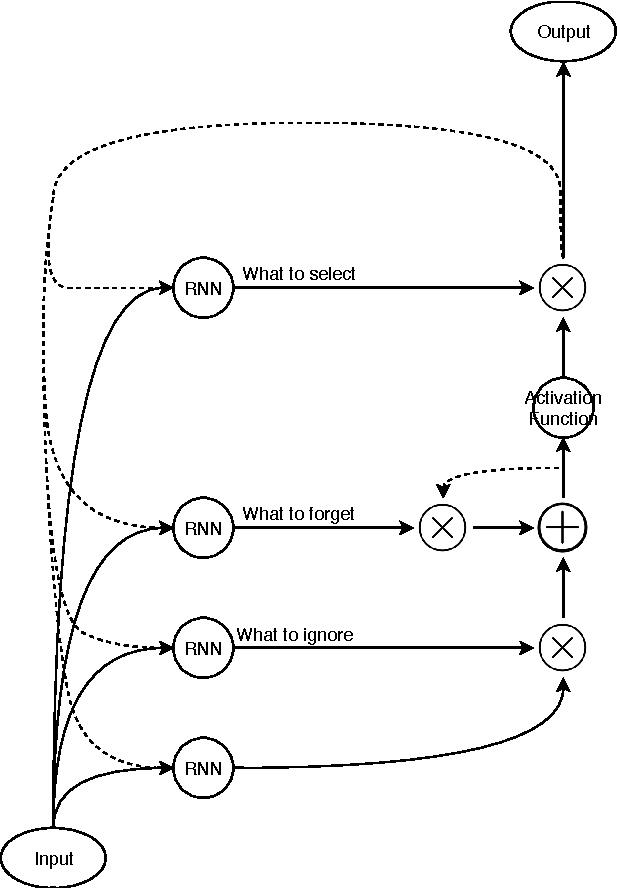
\includegraphics[scale=0.5]{./pictures/method/LSTM}
            \caption{The structure of an \gls{LSTM} network. $\bigoplus$ means
                an elementwise addition and $\bigotimes$ means an elementwise
                multiplication. Dotted lines show the movement of activations in
                the previous timestep while full lines show movement of the
                input in the current timestep.}
            \label{fig:lstm}
        \end{figure}

        The input to the \gls{LSTM} is fed into 4 \gls{RNN} networks that also
        receives the output from the previous timesteps. From bottom to top in
        the Figure the networks are:

        First: A network combining the current input and the previous output into
        an activation in the current timestep.

        Second: A network combining the current input and the previous output to
        compute which part of the activation of the first network to keep. The
        output of the second network is combined with the first network with an
        elementwise multiplication. That means that if the second network output
        a small value in a particular part of the output vector then that value
        will disappear from the output of the first network. The \gls{LSTM}
        therefore learns which part of the output to ignore.

        Third: A network combining the current input and the previous output
        to decide what to forget. The output of the network is combined with
        the current memory with an elementwise multiplication. So again if the
        network outputs a small value it can choose to forget a certain item.
        The network will learn when to throw things out of the current memory
        and when to keep them. The output of the elementwise multiplication is
        then combined with the current output via a elementwise addition. That
        allows the current memory to influence the output of the network. The
        added output and memory are transferred through an activation function
        that makes sure that nothing blows up and we get numerical instability.

        Fourth: A network combining the current input and the previous output
        to choose which values of the current output to select as the actual
        output. The output of the fourth network will be combined with the
        current model with an elementwise multiplication. So again the network
        can select which values to keep by outputting large numbers and which
        values to throw away by outputting small numbers. This network is the
        last applied to the output and can therefore select which values should
        be output.

        % TODO: cite http://www.bioinf.jku.at/publications/older/2604.pdf
        % Which is the original article for LSTMs.
        % Also cite http://www.cs.toronto.edu/~graves/preprint.pdf.

    \item[Embedding:]

        The embedding layer is a layer that maps a value into a continuous
        vector space. Given a sequence of integers, it uses the weights
        associated with the layer to map that singular value to a vector of
        predetermined size. This can be done on any sort of data, as longs as it
        is encoded as a sequence of integers. In \gls{NLP} circumstances, this
        can be applied to characters or words for example, where each element in
        the sequence is first encoded as an integer value, and then fed to the
        embedding layer, which maps it to the continuous vector space. The hope
        with using a layer such as this, that characters for example, get mapped
        to a point close to other similar characters. In addition it also adds
        another trainable layer to optimize on.

        \begin{figure}
            \centering
            \textbf{Example Character Embedding}\par\medskip
            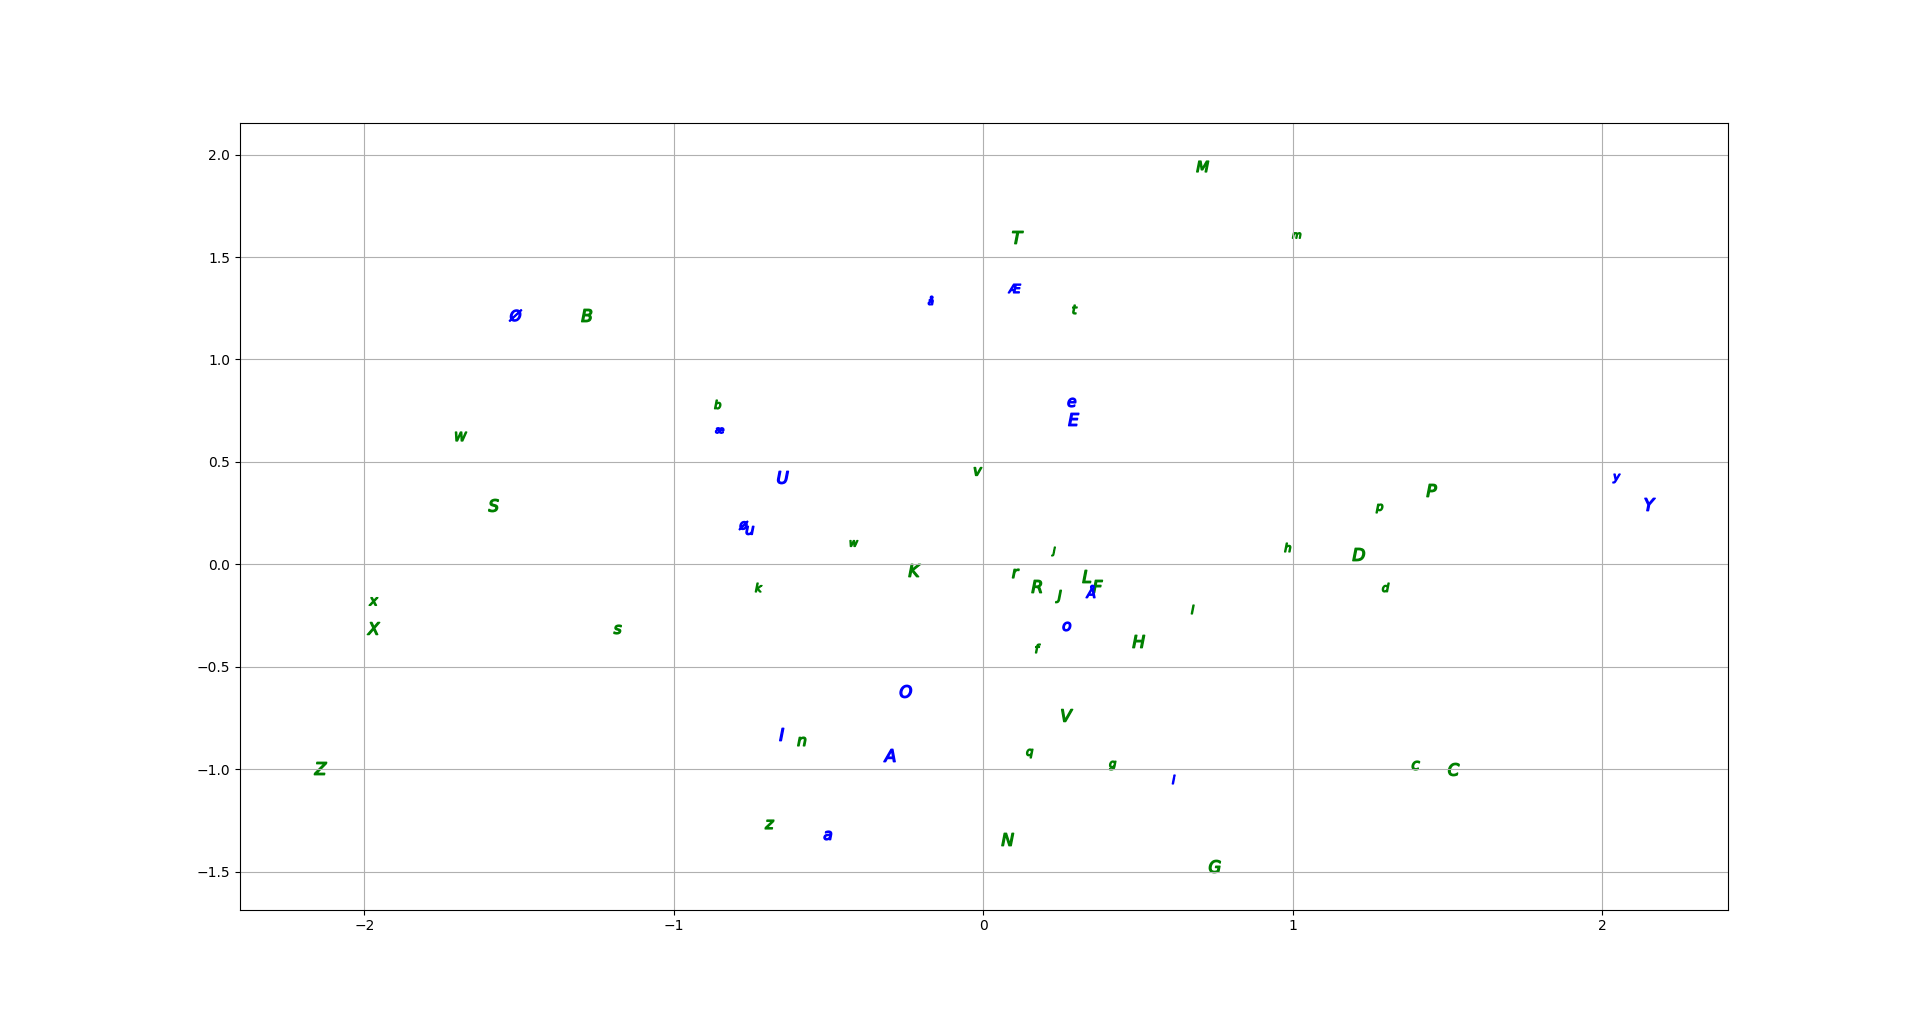
\includegraphics[width=\textwidth]{./pictures/method/example_character_embeddings.png}
            \caption{Character embeddings learned by a neural network. The
                embeddings were originally in 5 dimensional vectorspace and what
                is shown here is the first two principal components. Vowels are
                shown in blue and consonants in green.}
            \label{fig:embeddings}
        \end{figure}

        In Figure \ref{fig:embeddings} we have shown an embedding of one of our
        networks produces. The characters are embedded in 5 dimensions so the
        plot shows the first two principal components only. We can see that
        several lower and upper case letters have ended up close to each other.
        That means that the network has learned that those characters are
        interchangeable.

        Embedding layers are widely used in \gls{NLP}. They are mainly used
        to embed words in some vector space. \citet{mikolov2013linguistic}
        found that embedding layers are able to learn more that just word
        similarities. They for example found that $vec("king") - vec("man") +
        vec("woman") \approx vec("queen")$ that is the embeddings learned the
        relation between the words king and queen and not just that they are
        similar words.

    \item[Pooling Layer:]

        The purpose of a pooling layer, or down-sampling layer, is as the name
        suggest, to pool the data it receives. It does so with the goal of
        reducing the data down to a number a number of key features found within
        that same data. This of course decreases the computation time of the
        network as a whole, and with a smaller amount of parameters, comes a
        smaller chance of overfitting.

        Working in similar fashion as the convolutional layer, the max pooling
        layer also uses a sliding window. This sliding window of a certain
        dimensionality, is moved over the data given to it. The maximum value
        inside that window is then extracted, and determined to be the output
        for that specific placement of the window. The window then moved a
        specified stride size, and the process is repeated. The result is a
        dataset which is down-sampled in proportion with the sliding windows
        dimensions, and the stride. An example of this max pooling process can
        be seen in Figure \ref{fig:max_pool}.

        Pooling layers are however, not restricted to only the max pooling
        layer. The average pooling layers, works in a very similar fashion,
        but instead of extracting the max value, it simply averages values
        currently in the window. The Global Max Pooling Layer, which we use
        quite frequently in our networks does not use a window like the other
        ones described, but instead simply extracts the maximum value across
        the data the layer is provided, thus eliminating the need for a sliding
        window.

        \begin{figure}
        \centering
        \begin{equation}
            \begin{tabular}{|llll|}
            \hline
            1 & 8 & 7 & 2 \\
            9 & 7 & 9 & 8 \\
            3 & 6 & 2 & 4 \\
            5 & 7 & 9 & 9 \\\hline
            \end{tabular}
                \Longrightarrow
            \begin{tabular}{|ll|ll|}
            \hline
            \cc{blue}1 & \cc{blue}8 & \cc{red}7 & \cc{red}2 \\
            \cc{blue}9 & \cc{blue}7 & \cc{red}3 & \cc{red}8 \\ \hline
            \cc{orange}3 & \cc{orange}6 & \cc{green}2 & \cc{green}4 \\
            \cc{orange}5 & \cc{orange}7 & \cc{green}9 & \cc{green}9\\
            \hline
            \end{tabular}
                \Longrightarrow
            \begin{tabular}{|l|l|}
            \hline
            \cc{blue}9 & \cc{red}8\\\hline
            \cc{orange}7 & \cc{green}9\\
            \hline
            \end{tabular}
        \end{equation}
        \caption{An example of a max pooling performing using a 2x2 kernel and
            stride 2.}
        \label{fig:max_pool}
        \end{figure}


    \item[Dropout Layer:]

        The layer is used for regularization of neural networks. A good
        optimizer of a network will slowly fit more and more to the training
        data it is provided. This might seem like a bad thing at first, but if
        the validation error follows the training error as the network learns
        the training data, then the network is successfully learning some
        general commonality that can be used to describe both the data. It is
        the two errors do not follow on another that one has to be alarmed, as
        the network does not generalize properly. This is where the dropout
        layer is useful. By deactivating a certain amount of randomly selected
        neurons in a particular layer, the network is forced to learn from a
        larger sparse set of neurons, rather than focusing on a small amount
        of very informative ones. That typically results in a potential better
        understanding of the data as a whole rather than small amount of key
        features. An example of this can be seen in Figure \ref{fig:dropout}.

        \begin{figure}
            \centering
            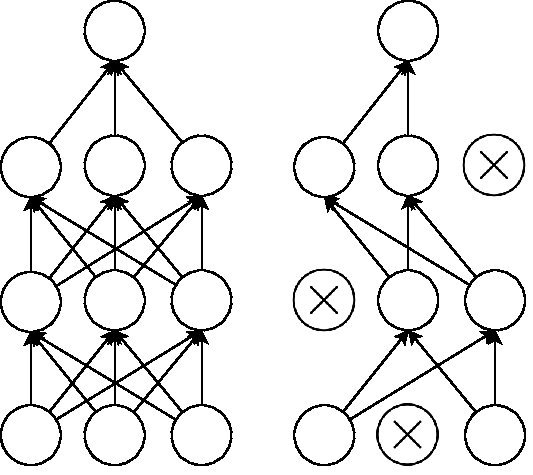
\includegraphics[width=0.5\textwidth]{./pictures/method/dropout}
            \caption{An example of the application of a dropouts being performed
                on different layers.}
            \label{fig:dropout}
        \end{figure}

        \citet{JMLR:v15:srivastava14a} investigated the use of dropout
        layers in different problem settings. They found that dropout layers
        reduced overfitting in all problems they looked at. In particular
        they found that document classification, which is similar to what we
        are doing was also improved. The main drawback of a dropout layer
        is that it increase the training time of the networks its used on
        \citep{JMLR:v15:srivastava14a}.

\end{description}


\subsubsection{Training a Network} \label{subsubsec:training_a_network}

A neural network learns by updating the weights in the network. The weights are
updated using \textit{gradient descent} \citep{Bishop}. Gradient descent is
a method that can minimize any differentiable function by taking small steps
towards a local minimum. The function we minimize in a neural network is an
error function. The error function describes a quantity that when minimized
gives the network the best performance possible. Since gradient descent works
for any differentiable function the error function can be any function that is
differentiable. As an example consider the \gls{MSE} function,

\begin{align}
    MSE(W)   &= \frac{1}{N} \sum_{n=1}^{N} MSE_n(W) \\
    MSE_n(W) &= \frac{1}{2} \left( \hat{y}_n - y_n \right)^2
\end{align}

where $N$ is the number of training samples, $\hat{y}_n$ is the predicted
results, $y_n$ is the target, and $W$ is a set of weights. That function is
often used to describe the error on networks with real valued output. The
gradient is a multi-variable generalization of the derivative of a function.
It is vector that points in the direction of steepest ascend in value for a
function at a specific point. Gradient descent is based on the observation that
a differentiable function $f$ in point $\mathbf{x}$ decrease fastest in the
direction of the negative gradient of the point $\mathbf{x}$ \citep{Bishop}.
That leads to a simple update rule that can be applied continuously to reach a
local minimum,

\begin{equation}
    \mathbf{x}_{n+1} = \mathbf{x}_n - \eta \Delta f\left(\mathbf{x}_n\right),
\end{equation}

where $\eta$ is a small number that makes sure we do not overstep the local
minimum. An example of the gradient descent process can be seen in Figure
\ref{fig:gradient_descent}. In terms of minimizing an error function in a neural
network by changing its weights $\mathbf{w}$ the gradient descent update rule
looks like,

\begin{figure}
    \centering
    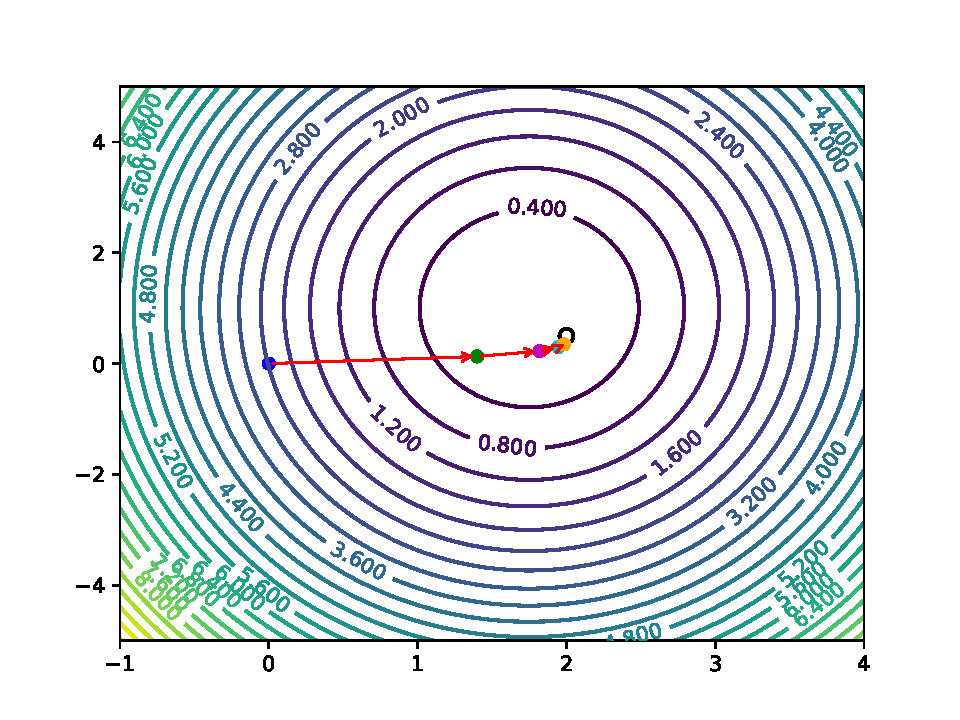
\includegraphics[width=0.8\textwidth]{./pictures/method/gradient_descend}
    \caption{An illustration of how gradient descent works. Each iteration steps
        in the direction of the global minimum of the specific function used,
        which in this case is signified by a black ring. The Figure is generated
        using code from
        \url{https://scipython.com/blog/visualizing-the-gradient-descent-method/}.}
    \label{fig:gradient_descent}
\end{figure}

\begin{equation} \label{eq:gradient_descent_network_update}
    \mathbf{w}^{(t+1)} = \mathbf{w}^{(t)} + \eta \Delta \mathbf{w}^{(t)},
\end{equation}

where $t$ is the timestep of the update and,

\begin{equation}
    \Delta \mathbf{w}^{(t)} = -\nabla E|_{\mathbf{w}^{(t)}}.
\end{equation}

$\nabla E|_{\mathbf{w}^{(t)}}$ refers to the gradient of the error function
relative to the specific weight vector $\mathbf{w}^{(t)}$, or rewritten,

\begin{equation}
    \nabla E|_{\mathbf{w}^{(t)}} = \frac{\partial E}{\partial \mathbf{w}^{(t)}}.
\end{equation}

Now we have an update rule for the weights of the network that will minimize
an error function $E$ chosen by us. We can choose $E$ as any function we want
that represent our target and is differentiable. The only problem left is how
to compute the gradient of the network. The computation of the gradient can be
done via the \gls{BP} algorithm \cite{Bishop}. \Gls{BP} depends on the
activation of all neurons to a specific sample. That gives us a three step
algorithm for updating the weights of the network.

\begin{description}
    \item[Feed Forward] Give input to first layer in network computing the
        activation of all neurons to that specific input.
    \item[Back Propagate] Use the \gls{BP} algorithm to compute the gradient of
        the network.
    \item[Update Weights] Use gradient descent to update the weights of the
        network.
\end{description}

The computation of the gradient starts at the error function $E$. If we for
simplicities sake focus on only a single training sample and fix $E$ as the
\gls{MSE}. We can compute the loss as follows,

\begin{equation}
    E = \frac{1}{2}(\hat{y} - y)^2.
\end{equation}

As mentioned we want to determine the gradient of this with respect to all the
weights in our network $w_{ij} \in W$. In order to do that we need to find
partial derivatives for those same weights and since each specific weight is
tied to a specific neuron we need to differentiate the entire network. But
before doing so, we need to establish the chain rule.

\begin{lemma}[Chain Rule]
\label{lemma:chainrule}

    If functions $f$ and $g$ are both differentiable and $F$ is the composite
    function defined by $F(x) = f(g(x))$, then $F' = f'(g(x)) \cdot g'(x)$,

\end{lemma}

The reason we need of the chain rule is that the loss function is essentially
a chain of function calls that spans the entire network. This fact becomes
apparent when we attempt to evaluate our single sample error function $E$ with
respect to a weight $w_{ij}$. If we keep in mind that the neurons in feed
forward neural networks computes a weighted sum of its inputs as per $a_i$ in
Equation \eqref{eq:neuron}. Then we known that $E$ only depends on $w_{ij}$
through the call of $a_i$, and it is for that reason what we can apply the chain
rule to get the following,

\begin{equation} \label{eq:bp_start}
    \frac{\partial E}{\partial \mathbf{w}_{ij}} = \frac{\partial E}{\partial a_i}
    \frac{\partial a_i}{\partial \mathbf{w}_{ij}}.
\end{equation}

We can add a little extra notation, which we will use hence forth, for the
sake of easing understanding,

\begin{equation}\label{eq:delta}
    \delta_i = \frac{\partial E}{\partial a_i}.
\end{equation}

$\delta$ is often referred to as the \textit{error} of a specific neuron.
From Equation \eqref{eq:neuron} we get that,

\begin{align}
    \frac{\partial a_i}{\partial \mathbf{w}_{ij}}
        &= \frac{\partial}{\partial \mathbf{w}_{ij}}
            \sum_{k=1}^d \mathbf{w}_{ik} x_k + \mathbf{w}_{i0}\\
        &= \frac{\partial}{\partial \mathbf{w}_{ij}} \sum_{k = 0}^d
            \mathbf{w}_{ik} x_k\\
        &= x_j.
\end{align}

Notice that we exchanged the $j$ counter in Equation \eqref{eq:neuron} with $k$
since we would otherwise have a name clash. That equation when combined with
Equation \ref{eq:bp_start} gives us,

\begin{equation} \label{eq:deriv}
    \frac{\partial E}{\partial \mathbf{w}_{ij}} = \delta_i x_j.
\end{equation}

That reveals that the derivative of the cost function with respect to the weight
$\mathbf{w}_{ij}$ is simply the value of $\delta$ for the neuron at the output
end and $x$ for the input end of the weight for that same neuron. This leaves us
with calculating $\delta_i$ for the hidden units, and the output units of the
network. We already know that for output units $\delta$ is computed as,

\begin{equation}
    \label{eq:output}
    \delta_k = \hat{y}_k - y_k,
\end{equation}

where $k$ refers to a specific output neuron. For the hidden units the chain
rule has to be used again,

\begin{equation}
    \label{eq:bp}
    \delta_i = \frac{\partial E}{\partial a_i} =
    \sum_k \frac{\partial E}{\partial a_k} \frac{\partial a_k}{\partial a_i},
\end{equation}

Where the sum runs over all $k$ output units from unit $i$. The Equation can be
rewritten using the prior established equalities and the chain rule,


\begin{align}
    \sum_k \frac{\partial E}{\partial a_k} \frac{\partial a_k}{\partial a_i}
    &= \sum_k \delta_k \frac{\partial a_k}{\partial a_i}
    & \text{By Equation \eqref{eq:delta}}
    \\
    &= \sum_k \delta_k \frac{\partial a_k}{\partial z_i}
        \frac{\partial z_i}{\partial a_i}
    & \text{By Equation \eqref{eq:neuron} and Lemma \ref{lemma:chainrule}}
    \\
    &= \sum_k \delta_k h'(a_i) \frac{\partial a_k}{\partial z_i}
    \\
    &= \sum_k \delta_k h'(a_i) \left( \frac{\partial}{\partial z_i}
        \sum_{j} \mathbf{w}_{kj} z_j\right)
    \\
    &= \sum_k \delta_k h'(a_i) \mathbf{w}_{ki}
    \\
\end{align}

This highlights that changes in $a_i$ only influences the error-function,
through variations of the variables $a_k$. We can compute the $\delta$ for a
particular hidden unit by backpropagating the $\delta$ value back from higher up
in the network.

As such, we can summarize the weight updating algorithm as,

\begin{enumerate}
    \item

        Provide the network with some input data $x_n$, and compute the
        activations of each hidden and output neuron using Equation
        \eqref{eq:neuron},

    \item

        Compute $\delta_n$ for each of the output neurons using Equation
        \eqref{eq:output},

    \item

        Back propagate $\delta$s using Equation \eqref{eq:bp} to compute
        $\delta_i$ for each neuron,

    \item

        Use Equation \eqref{eq:deriv} to evaluate the required derivatives.

    \item

        Update the weight using the computed derivatives
        and the gradient descent update rule from Equation
        \eqref{eq:gradient_descent_network_update}.

\end{enumerate}

% TODO: We should read through this paragraph and rewrite it a bit. It is a bit
% hard to read.

These three steps feed forward, backpropagate and update weights are repeated
throughout the training cycle of the neural networks. Such that the weights
are optimized after each full parse over the training dataset. As is to be
expected this algorithm as very expensive computationally as it runs in $O(W)$.
This is only for a single training sample though. Thus run-time becomes $O(N
\cdot W)$, where $N$ is the number of training samples. Additionally, if
one trains over several epochs, this run-time becomes even more inflated
with $O(\mathcal{E}\cdot N\cdot W)$ iterations having do be computed, where
$\mathcal{E}$ is the number of epochs run during training. For that reason
this run-time might not seem very viable at first, and is indeed the reason
why neural networks need such a long training time. However an alternative
described by \citet{Bishop}, which involves perturbing each weight instead, and
approximating the derivatives. This method does however run in $O(W^2)$ time,
making the run-time of $O(W)$ backpropagation provides the desired choice.
However, in order to improve on those that $O(W)$ time-complexity a method
called batching is used. This method, shuffles and split the training dataset
up into smaller batches. These batches are then run through the network one at
a time, performing backpropagation after each run-through. This results in the
gradient not being as accurate after each batch, but this introduced inaccuracy
is negligible compared to the computational time won, by reducing the amount of
$\mathcal{E}$ in $O(\mathcal{E}\cdot N\cdot W)$ needed for the same amount of
convergence. A mote detailed description of this process can be found in the
next Section. \citep{Bishop}.


\subsubsection{Optimizers}\label{sec:optimizers}

Traditional gradient descent has been updated with several different algorithms.
These algorithms are called \textit{optimizers}. A good optimizer algorithm
will reach a local minimum faster than traditional gradient descent. The first
optimizer algorithm we will discuss is the \textit{stochastic gradient descent}
algorithm. In the traditional gradient descent we have described a single
weight update require computing the gradient of the error function on each
training sample. Often such a detailed gradient is not needed in practise.
Stochastic gradient descent is an attempt at estimating the gradient of all
datapoints using only a single datapoint. That means that in stochastic gradient
descent weights are updated much more often and is updated on a noisy target
\citep{Bishop}. The advantage of stochastic gradient descent is that convergence
to a local minimum might be much quicker since the algorithm does not have to
go through all training samples for each weight update. The weight updating for
stochastic gradient descent is computed as,

\begin{equation}
    \mathbf{w}^{(t+1)} =
        \mathbf{\mathbf{w}}^{(t)} -
        \eta\Delta E_n|_{\mathbf{w}^{(t)}}.
\end{equation}

In practise each weight update in stochastic gradient descent are computed
not based on a single training sample but on some small number of training
samples. That allows the computation to take advantage of highly optimized
matrix libraries and making each update on a slightly less noisy target
\footnote{\url{http://ufldl.stanford.edu/tutorial/supervised/OptimizationStochas
ticGradientDescent/}}. The version of stochastic gradient descent that use more
than one sample per weight update is known as stochastic minibatch gradient
descend.

To see how stochastic gradient descent might lead to faster convergence consider
a dataset with some number of training samples. To create redundancy in the
dataset we copy all training samples in the dataset to create a new dataset of
twice the size. In classical gradient descent the only effect will be that the
error increases by a magnitude of 2 but will take twice as long to compute.
While stochastic gradient descent will converge at the exact same speed as each
minibatch will still represent an estimate of the true underlying function and
each weight update still takes the same amount of time \citep{Bishop}.

Another advantage of the stochastic method is that the optimizer might escape
from a non optimal local minima and reach a better local minima. To see why that
might happen consider the fact that each minibatch consist of a different sample
of training samples. Even though when computed on all training samples the
gradient points towards the non-optimal local minima the gradient of a single
batch might point towards a better local minima. Therefore the optimizer has the
possibility of following the gradient of single batches that leads to a final
better local minima \citep{Bishop}.

A problem in the stochastic gradient descent algorithm is the need to choose
the learning rate $\eta$. If the learning rate is too high the algorithm
will diverge and if it is to low it will be very slow to converge. Therefore
several extensions to basic stochastic gradient descent has been developed that
automatically tunes the learning rate $\eta$. We will discuss three different
extension \gls{AdaGrad}, \gls{RMSProp} and \gls{Adam}.

In the description of those three algorithms we will slightly abuse vector
notation. Given $\mathbf{a}, \mathbf{b} \in \mathbb{R}^n$ we will keep using
$\mathbf{a} \otimes \mathbf{b}$ to mean an elementwise multiplication but
besides that we use $\frac{\mathbf{a}}{\mathbf{b}}$ to mean an elementwise
division, $\sqrt{\mathbf{a}}$ to mean an elementwise square root and
$\mathbf{a}^n$ to mean an elementwise power.

\begin{description}

    \item[\gls{AdaGrad}:]

        The algorithm was invented by \citet{Duchi:2011:ASM:1953048.2021068}.
        The algorithm attempts to solve the problem of choosing a learning
        rate and the problem of how to handle parameters that are infrequently
        activated. When a parameter is only infrequently activated the gradient
        on that parameter will often be close to 0. Infrequently used parameters
        are often the most important parameters for a classification task but
        since they are infrequent they are hard to learn on. \gls{AdaGrad}
        assigns a separate learning rate to each separate parameter. The
        algorithm gives infrequently observed parameters a very high learning
        rate and frequently observed parameters a very low learning rate. The
        method incorporates knowledge of the data from previous iterations to
        make choices in the current iteration. In \gls{AdaGrad} the weight
        update function is,

        \begin{equation}
            \mathbf{w}^{(t+1)} =
                \mathbf{w}^{(t)} -
                \eta \text{diag}\left(G^{(t)}\right)^{-\frac{1}{2}} \otimes
                \Delta E|_{\mathbf{w}^{(t)}},
        \end{equation}

        where $G^{(t)}$ is a matrix containing the sum of the outer product
        of the gradient in all previous timesteps $1, \dots, t$ and
        $\text{diag}(X)$ is the diagonal vector of the matrix $X$. $G^{(t)}$ is
        defined as,

        \begin{equation}
            G^{(t)} = \sum_{t'=1}^t \Delta E|_{\mathbf{w}^{(t')}}
                \left(
                    \Delta E|_{\mathbf{w}^{(t')}}
                \right)^T.
        \end{equation}

        For the updating of a single weight $w_i$ the above becomes
        \citep{Duchi:2011:ASM:1953048.2021068},

        \begin{equation}
            \label{eq:individual_adagrad}
            \mathbf{w}_i^{(t+1)} =
                \mathbf{w}_i^{(t)} - \frac{\eta}{\sqrt{G^{(t)}_{ii}}} \otimes
                \Delta E|_{\mathbf{w}_i^{(t)}}.
        \end{equation}

        $G_{i,i}$ works as a scaling factor for weight $\mathbf{w}_i$.
        Since $\sqrt{G_{ii}} = \sqrt{\sum_{t'=1}^t \left(\Delta
        E|_{\mathbf{w}^{(t')}_i}\right)^2}$, $G_{i,i}$ is the L2 norm
        of the gradient in the previous timesteps. That means that if the
        gradient has generally been large for a particular weight the norm
        will be large and the updating of the weight will be scaled down
        (slower) which can be seen in Equation \eqref{eq:individual_adagrad}.
        Similarly when the gradients of a weight has been small or 0 the
        weight is scaled less down and the upgrade will be larger. That has
        the effect of having infrequent parameters of the model train faster
        \citep{Duchi:2011:ASM:1953048.2021068}.

        % TODO: Describe why AdaGrad is great for NLP.

    \item[\gls{RMSProp}:]

        \gls{RMSProp} was introduced by Geoff Hinton in lecture 6e of his
        Coursera Class \citep{DBLP:journals/corr/Ruder16}. This section is based
        primarily on his slides \citep{HintonSrivastavaSwersky2014}. The idea
        behind \gls{RMSProp} is similar to \gls{AdaGrad} each weight is updated
        at an independent rate. Unlike \gls{AdaGrad} the rate is chosen by a
        moving average instead of the L2 norm of all previous steps. That allows
        the algorithm to adapt quickly to changes in the gradient. When the
        gradient of a weight is large the algorithm decreases the learning rate
        and when the gradient is consistently small it tunes up the learning
        rate. That functions well since a large gradient is found in a steep
        volatile area while a consistently small gradient is found in a flat non
        volatile area. In the steep areas we are likely to overshoot the target
        if the learning rate is to high while in flat areas we do not have that
        problem. The internal state of the algorithm is a vector $\mathbf{v}$
        of the running average of gradient magnitudes. It is updated with the
        equation,

        \begin{equation}
            \label{eq:rms_prop_state}
            \mathbf{v}^{(t+1)} =
                \gamma\mathbf{v}^{(t)} +
                (1 - \gamma)\left(
                    \Delta E|_{\mathbf{w}^{(t + 1)}} \otimes
                    \Delta E|_{\mathbf{w}^{(t + 1)}}
                \right).
        \end{equation}

        The parameter $\gamma$ can be seen as a remembering rate. If $\gamma$
        is high we keep much of the previous running average and if $\gamma$
        is low we update the average much quicker. The actual weight update is
        performed by using the internal state $\mathbf{v}$ to scale the learning
        rate $\eta$,

        \begin{equation}
            \mathbf{w}^{(t+1)} =
                \mathbf{w}^{(t)} -
                \frac{\eta}{\sqrt{\mathbf{v}^{(t)}}} \otimes
                \Delta E|_{\mathbf{w}^{(t)}}.
        \end{equation}

    \item[\gls{Adam}:]

        \gls{Adam} is an upgrade of the \gls{RMSProp} algorithm invented by
        \citet{DBLP:journals/corr/KingmaB14}. The difference from \gls{RMSProp}
        is that \gls{Adam} use both the gradient and the squared gradient while
        \gls{RMSProp} use only the squared gradient. Consequently \gls{Adam} has
        two remembering factors instead of the single one for \gls{RMSProp}. The
        internal state of \gls{Adam} is updated via,

        \begin{align}
            \mathbf{m}^{(t+1)} &=
                \gamma_1\mathbf{m}^{(t)} +
                (1 - \gamma_1) \Delta E|_{\mathbf{w}^{(t+1)}}, \\
            \mathbf{v}^{(t+1)} &=
                \gamma_2\mathbf{v}^{(t)} +
                (1 - \gamma_2) \left(
                    \Delta E|_{\mathbf{w}^{(t+1)}} \otimes \Delta E|_{\mathbf{w}^{(t+1)}}
                \right), \\
            \mathbf{\hat{m}}^{(t+1)} &=
                \frac{\mathbf{m}^{(t+1)}}{1 - \gamma_1^{t + 1}}, \\
            \mathbf{\hat{v}}^{(t+1)} &=
                \frac{\mathbf{v}^{(t+1)}}{1 - \gamma_2^{t + 1}}.
        \end{align}

        The first two equations are very similar to Equation
        \eqref{eq:rms_prop_state} for \gls{RMSProp}. In those equations
        $\gamma_1$ and $\gamma_2$ are the decay rates of the gradient and the
        squared gradient. They keep a running average of the gradient and the
        size of the gradient. By using the running average of the gradient
        \gls{Adam} is able to move more smoothly in a direction since the
        direction chosen is no longer just the current gradient but previous
        gradients influence the choice of direction. That means that a single
        weird gradient will not drastically change the direction \gls{Adam}
        moves \citep{DBLP:journals/corr/KingmaB14}. Similarly to \gls{RMSProp}
        \gls{Adam} use the running average of the squared gradient to scale how
        large steps are taken. The two bottom equations are scaling the internal
        state based on the time step $t$. As $t$ increases the denominators
        increase meaning that the value of the whole fraction decreases. That
        means that in the beginning the step size is adjusted upwards and as
        $t$ increases, smaller and smaller steps are taken. The actual weight
        updates in the \gls{Adam} algorithm are then given by,

        \begin{equation}
            \mathbf{w}^{(t + 1)} = \mathbf{w}^{(t)} -
                \eta\frac
                    {\mathbf{\hat{m}}^{(t+1)}}
                    {\sqrt{\mathbf{\hat{v}}^{(t+1)}} + \epsilon}.
        \end{equation}

        \gls{Adam} prevents division by 0 via the $\epsilon$ parameter which is
        just some small number. It can be seen in the above equation that the
        direction of change is chosen by $\mathbf{\hat{m}}^{(t)}$ while the size
        of the step taken is chosen by a combination of the learning rate $\eta$
        and $\mathbf{\hat{v}}^{(t)}$.

\end{description}


\subsubsection{Siamese Networks}\label{subsubsec:siamese_networks}

Classical machine learning approaches for text analysis and all our baseline
methods are based on handcrafted feature sets. Deep learning has shown
promising results in extracting features from raw images and raw text
\citep{hongxiaosunyuan}. We wanted to use deep learning to automatically
learn features from a large amount of data. At the same time we want to solve
the MaCom problem. Siamese neural networks are as described earlier networks
that compares two inputs. They have been used for comparing texts, images and
signatures \citep{Koch2015SiameseNN,NIPS1993_769,qian:2018}. \citet{qian:2018}
use a Siamese network but with no convolutions and a distance function on top
for text analysis while \citet{Koch2015SiameseNN} used a siamese network with
convolutions and fully connected network on top for image analysis. Our approach
is to use convolutions or \gls{RNN}s in the siamese network to learn important
features from the texts. We also use a fully connected network on top of the
feature extraction layers to learn from the features the extracted. An example
of this architecture can be seen in Figure \ref{fig:siamese_example}.

\begin{figure}
    \centering
    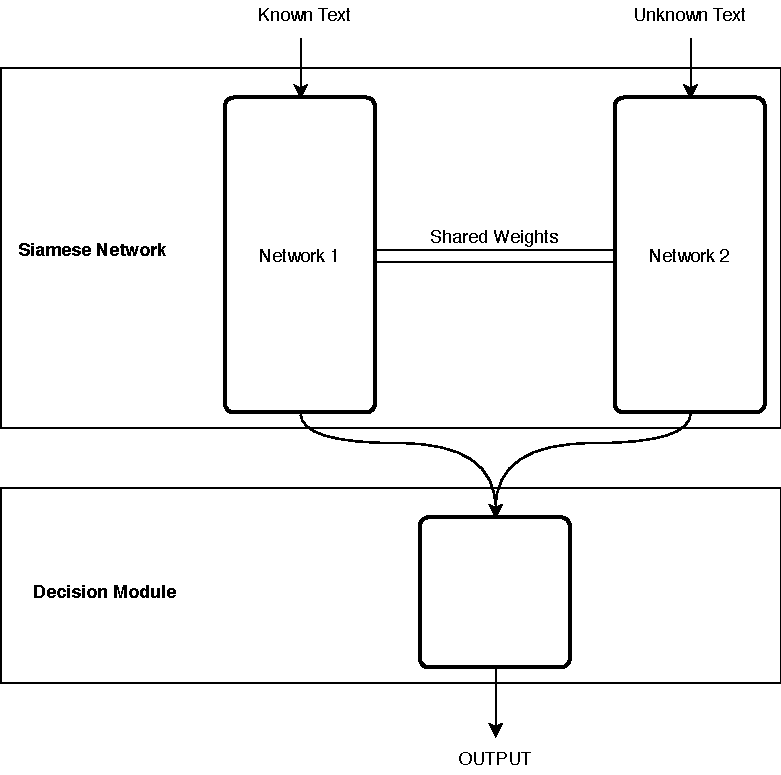
\includegraphics[scale=0.5]{./pictures/method/siamese}
    \caption{The basic architecture of a siamese neural network. The network
        takes two sources of data and runs it through two parallel weight
        sharing networks. The two parallel networks extracts features from the
        raw data. Those features are given to a prediction module that compares
        the feature sets extracted. The decision module can be anything that
        compares two vectors such as a distance function or a dense neural
        network.}
    \label{fig:siamese_example}
\end{figure}

The network will take two inputs, a text $t \in T_\alpha$ and a text $t' \in
T_{\alpha'}$. The network will then try to determine whether $\alpha = \alpha'$
by comparing $t$ and $t'$. The texts will be represented in some format such as
a sequence of characters or a sequence of words. The siamese part of the network
will extract features from the texts using convolutions or \gls{RNN} layers.
These features will serve as a \textit{representation} of the texts $t$ and
$t'$. This representation will be given to some dense layers which will learn
how to compare the feature sets extracted.

\citet{DBLP:journals/corr/0001KYS17} presented a comparative study of
\glspl{CNN} and \glspl{RNN} in common \gls{NLP} tasks. They found that
\glspl{RNN} generally performed better in tasks where understanding the whole
text was important while \glspl{CNN} performed better when understanding was
secondary and the goal was mainly about finding key phrases or statistical
information from a text. In authorship verification the understanding of the
text is generally irrelevant since we do not have to say anything about what a
text is about but only whether or not it is written by the same author as some
other text. Furthermore classical authorship verification methods have relied
on statistical information from the texts and not on an actual understanding of
the texts. We have therefore chosen to start out with using convolutional neural
networks.

The final output of the networks we train will be the probability that $\alpha =
\alpha'$. Since the MaCom dataset consist of multiple texts per author and this
network architecture only compares two texts we define a separate system for
making the final prediction based on all the known texts of an author.


\subsection{Combining Neural Network Output}
\label{subsec:combining_neural_network_output}

In the generic Siamese \gls{NN} presented in Section
\ref{subsubsec:siamese_networks} the output of the network is a probability
that two texts are written by the same author. However in the problem we are
trying solve defined in Definition \ref{def:authorship_verification} we take
several texts as input. We therefore need a method of combining the predictions
on multiple texts to a single prediction on a particular problem instance.
We do that using a \textit{prediction system}. We let the generic siamese
\gls{NN} described above be known as a \textit{text comparison function} $f \in
\mathcal{F}$.

\begin{definition}[Text Comparison Function]
    \label{def:text_comparison_function}

    Let $\mathcal{F} \colon \mathcal{T} \times \mathcal{T} \rightarrow [0, 1]$
    be any function that compares two texts and outputs the probability that the
    the texts are written by the same author.

\end{definition}

For fixed text comparison function $f$, we now define the \textit{weighted
average based prediction system} $P_w$.

\begin{definition}[Weighted Average Prediction System]
    \label{def:weighted_average_prediction_system}

    Let $w: \mathcal{T} \rightarrow [0, 1]$ be a weight function, such that
    $\forall \alpha \in \mathcal{A}: \sum_{t \in T_\alpha} w(t) = 1$. Then the
    weighted average prediction system is given by,

    \begin{align}
        &P_w \colon \mathcal{A} \times \mathcal{T} \times [0, 1] \rightarrow
            \{0, 1\} \\
        &P_w(\alpha, t, \theta) \mapsto \mathbbm{1}\left[
                \sum_{t' \in T_\alpha} w(t') f(t, t') > \theta
            \right],
    \end{align}

    where $\mathbbm{1}\left[\cdot\right]$ is the indicator function.

\end{definition}

That is, the weighted average prediction system $P_w$ returns 1 if the weighted
average of the probability that $t$ is written by the same author as $t'$ for
each $t' \in T_\alpha$ is greater than the threshold $\theta$ and 0 otherwise.

The $\theta$ parameter in $P_w$ determines when we consider an unknown text
to be written by an author. The $\theta$ parameter can be used to enforce how
sure we have to be of a decision to accuse an author of not having written
an assignment. As described earlier MaCom does not want to accuse innocent
students of cheating. That means that it is very important to MaCom to minimize
the accusation error. We can use the $\theta$ parameter to control that error.
Hopefully the \glspl{FN} will generally end up with a value closer to 1 than
the \glspl{TN}. If that is the case then lowering $\theta$ value will lower the
fraction since there will be fewer \glspl{FN}. That might lower the overall
accuracy of the prediction system but will make sure that at few students as
possible are falsely accused.

The $w$ parameter in the prediction system can be used to weigh the known
texts differently. We are going to try several different weight functions
that weigh texts based on metadata such as the time they were written and the
length of the texts. In the following definition of different weight functions
we will ignore the constraint that the weight functions has to sum to 1 for
each author. We ignore that constraint since for any weight function $w \colon
\mathcal{T} \rightarrow \mathbb{R}$ we can define a new weight function $w^*
\colon \mathcal{T} \rightarrow [0, 1]$ as,

\begin{equation}\label{eq:normalize}
    w^*(t) = \frac{w(t)}{\sum_{t' \in T_\alpha} w(t')}.
\end{equation}

We can therefore define the weight functions $w$ while ignoring the constraint
but use $w^*$ as the actual weight function in the weighted prediction system.

The most obvious weighing scheme is to just use a uniform weighting. That way
we simply take an average of the predictions of our networks over the different
texts an author has written.

\begin{definition}[Uniform Weight]
    \label{def:uniform_weight}

    The uniform weight function is given by,

    \begin{align}
        &u \colon \mathcal{T} \rightarrow \{ 1 \} \\
        &u(t) \mapsto 1.
    \end{align}

\end{definition}

The \textit{uniform weight} function does not use any information we know about
the texts. We define it as a baseline to make sure we do not make any weight
functions that are worse than a simple uniform weighing. Our other weight
functions makes use of metadata we know about the texts. We start by defining a
weight function \textit{exponential dropoff weight} that use the time a text was
turned in to MaComs servers to weight the texts. We assume that newer texts will
better reflect the current writing style of a student than older texts. Recall
that $\tau$ denotes the function that returns the relative time of a text as
described in Section \ref{subsec:notation}.

\begin{definition}[Exponential Dropoff Weight]
    \label{def:exponential_dropoff_weight}

    Given $\lambda \in \mathbb{R}^+$ the time based exponential dropoff weight
    function is given by,

    \begin{align}
        &exp_\lambda \colon \mathcal{T} \rightarrow \mathbb{R}^+ \\
        &exp_\lambda(t) \mapsto e^{-\lambda \tau(t)}.
    \end{align}

\end{definition}

The $\lambda$ parameter can be used to control how important newer texts are.
When $\lambda = 0$ the exponential dropoff weight is equivalent to the Uniform
Weight function and as $\lambda \rightarrow \infty$ more weight is given to the
most recent text. We have shown the weights given to different assignments for
different $\lambda$ values in Figure \ref{fig:weights}.

\begin{figure}
    \centering
    \textbf{Exponential Dropoff Weights}\par\medskip
    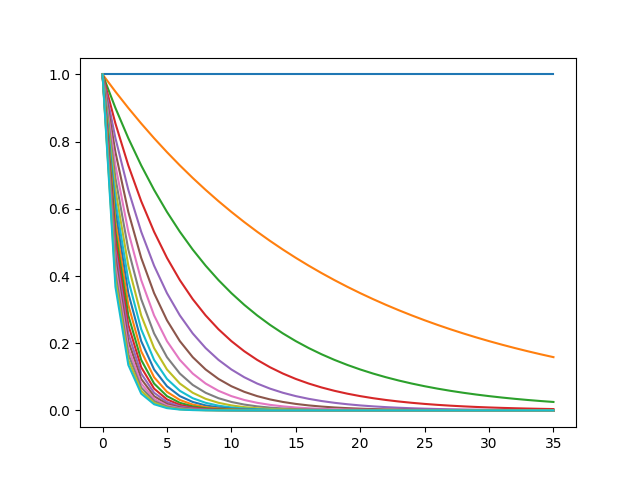
\includegraphics[width=0.49\textwidth]{./pictures/method/weights.png}
    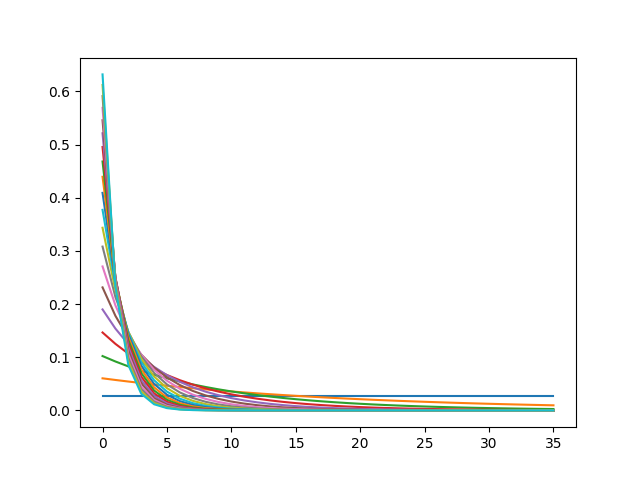
\includegraphics[width=0.49\textwidth]{./pictures/method/weights_normalized.png}
    \caption{Illustrate the Exponential Dropoff weight function for different
        values of $\lambda$. We apply the weight function to the numbers $0, 1,
        \dots, 35$ since a typical student will attend secondary school for 3
        years (36 months). On the left the pure output of the weight function
        $w_e$ is shown and on the right the normalized weights $w_e^*$. We wary
        $\lambda$ from 0 to 1 with step size 0.05.}
    \label{fig:weights}
\end{figure}

We have also defined weight functions that use other metadata besides the time
of writing. Specifically we have used the length of texts. The idea is that
longer texts provide better insight into an authors writing style than shorter
texts. So we wanted to see if we could obtain better results if we considered
text length.

\begin{definition}[Length Weight]

    The text length based weight function is given by,

    \begin{align}
        &l \colon \mathcal{T} \rightarrow \mathbb{N}^+ \\
        &l(t) \mapsto \left\lfloor \frac{|t|}{1000} \right\rceil + 1,
    \end{align}

    where $\lfloor x \rceil$ is $x$ rounded to nearest whole number.

\end{definition}

Thus this weight function gives more weight the longer a text is but where only
differences on the order of thousands of characters are considered significant.
We used the exponential dropoff weight and length weight functions to implement
another weight function that use both text length and time to give weights to an
assignment. The combined weight function is shown below.

\begin{definition}[Exponential Dropoff and Length Weight]

    Given $\lambda \in \mathbb{R}^+$ the combined time and length weight
    function is given by,

    \begin{align}
        &lexp_\lambda \colon \mathcal{T} \rightarrow [0, 2] \\
        &lexp_\lambda(t) \mapsto epx^*_\lambda(t) + l^*(t).
    \end{align}

\end{definition}

Which is simply the addition of the exponential dropoff weight and the length
weight, after they are both individually applied to the text.

We have also defined some different prediction systems that are not based on
weighted averages. The first such system is the $P_{max}$ prediction system.
The thought behind the system is that we wanted to minimize the accusation
error. The prediction system takes the text $t' \in T_\alpha$ that looks the
most like $t$. That way if just a single assignment from a candidate author
looks sufficiently like the text we are comparing with we report that the author
matches. That should hopefully result in less people being accused of ghost
writing.

\begin{definition}[Maximum Prediction System]
    \label{def:maximum_prediction_system}

    The maximum prediction system $P_{max}$ based only on most similar text is
    given by,

    \begin{align}
        &P_{max} \colon \mathcal{A} \times \mathcal{T} \times [0, 1] \rightarrow
            \{0, 1\} \\
        &P_{max}(\alpha, t, \theta) \mapsto \mathbbm{1}\left[
                \underset{t' \in T_\alpha}{\text{maximize}} f(t, t') > \theta
            \right].
    \end{align}

\end{definition}

For completeness we also defined a $P_{min}$ that use only the least similar
text for the prediction. We expect that such a function will be quick to accuse
authors of ghost writing since it only looks at the one text that seem to
indicate ghost writing.

\begin{definition}[Minimum Prediction System]
    \label{def:minimum_prediction_system}

    The minimum prediction system $P_{min}$ based only on least similar text is
    given by,

    \begin{align}
        &P_{min} \colon \mathcal{A} \times \mathcal{T} \times [0, 1] \rightarrow
            \{0, 1\} \\
        &P_{min}(\alpha, t, \theta) \mapsto \mathbbm{1}\left[
                \underset{t' \in T_\alpha}{\text{minimize}} f(t, t') > \theta
            \right].
    \end{align}

\end{definition}

Finally we also defined prediction system that takes a majority vote. The
majority vote is similar to a uniform weight function. The difference is that
the majority vote does not use the actual value of a prediction but only how
many are on each side of a threshold. As an example assume that an author
$\alpha$ has written three texts $\{t_1, t_2, t_3\} = T_\alpha$ and we are
comparing to text $t$ with $\theta = 0.5$. Let us then assume that $f(t, t_1) =
0.0$, $f(t, t_2) = 0.51$ and $f(t, t_3) = 0.51$. Then the uniform weight
function would compute $\mathbbm{1} \left[ \frac{1}{3} 0.0 + \frac{1}{3} 0.51 +
\frac{1}{3} 0.51 > 0.5 \right] = 0$. Meaning that the author would be accused of
using a ghost writer even though two of his assignments are more similar than
dissimilar. Contrary to that a majority vote would report 1 since more
texts are greater than $\theta$ than lower.

\begin{definition}[Majority Vote Prediction System]
    \label{def:majority_vote_prediction_system}

    The majority vote prediction system $P_{MV}$ is given by,

    \begin{align}
        &P_{MV} \colon \mathcal{A} \times \mathcal{T} \times [0, 1] \rightarrow
            \{0, 1\} \\
        &P_{MV}(\alpha, t, \theta) \mapsto \mathbbm{1}\left[
                \frac{1}{|T_\alpha|} \sum_{t' \in T_\alpha} \mathbbm{1}\left[
                    f(t, t') > \theta
                \right] > \frac{1}{2}
            \right].
    \end{align}

\end{definition}

% TODO: Write about error functions.
